\documentclass[xcolor=dvipsnames,slidestop,compress,mathserif, 11pt]{beamer}
\usecolortheme[named=Blue]{structure}
\usetheme[height=2mm]{Rochester}
\setbeamerfont{structure}{shape=\itshape}
\mode<presentation> {
\usetheme{Darmstadt} % Tema seleccionado.
\usecolortheme{default}%{albatross} % Color del tema.
\setbeamercovered{transparent} % Transparencia.
}
%\setbeamercovered{transparent}
%}%%%% packages y comandos personales %%%%
\setbeamertemplate{caption}[numbered]
\usepackage{ragged2e}
\usepackage{comment}
\renewcommand{\figurename}{Figura}
\renewcommand{\tablename}{Tabla}
%\usepackage{latexsym} % S��mbolos
\usepackage{amsmath}
\usepackage{array}
\usepackage{amssymb}
\usepackage{wasysym}
\usepackage{stmaryrd}
\usepackage{wrapfig}
\usepackage{multicol}
\usepackage{dsfont,float}
\usepackage{soul}
\usepackage{upgreek}
\usepackage{accents}
\usepackage{physics}
%\usepackage[lite]{mtpro2}
\usepackage{tikz}
\usepackage{lipsum}
\newcommand\Fontvi{\fontsize{6}{7.2}\selectfont}
%\usepackage{turnstile}
\font\shi=cmssdc10 scaled 700
\title[Tesis profesional]{Evoluci\'on de una funci\'on de Wigner de un amplificador param\'etrico}
\author{TESIS PROFESIONAL\\
Carlos Eduardo González Anguiano}
\institute{Departamento de Física ESFM-IPN}
\date{1 de junio de 2024}
\usepackage{graphicx}
%\graphicspath{%
%
%    {E:/Efi1-ggg/}% inserted by PCTeX
%    {/}% inserted by PCTeX
%}
\usepackage[utf8]{inputenc} % Usar latin1 causa error para acentos
\begin{document}


\maketitle


\begin{frame}
	\frametitle{Índice}
	\tableofcontents[pausesections]
\end{frame}

\section{Introducción}

\begin{frame}[c]
	\frametitle{Introducción: Mecánica Cuántica (MC)}
	\textbf{Max Planck y la \textit{catástrofe ultravioleta}}\\
	\justifying \textit{Densidad espectral de energía}: Energía por unidad de volumen de ondas electromagnéticas de frecuencia $\nu$.
	\begin{equation}
		u(T)=\int_{0}^{\infty}\rho(\nu, T)d\nu.
	\end{equation}
	\justifying La densidad de \textit{cuerpo negro} dado por termodinámica clásica difiere de datos experimentales.
	Planck propone estados de energía de osciladores discretos
	\begin{equation}
		E_n = nh\nu.
	\end{equation}
	\justifying La cuantización lleva a la \textit{distribución de Planck}
	\begin{equation}
		\rho(\nu, T) = \frac{\hbar \nu^3}{\pi^2 c^3} \frac{1}{e^{\hbar\nu/kT}-1}.
	\end{equation}
\end{frame}

\begin{frame}
	Figura de la distribución de Planck
\end{frame}

\begin{frame}
	\textbf{Einstein y el \textit{efecto fotoeléctrico}}\\
	\justifying Describe el efecto de la luz incidente sobre un metal, y como este emite electrones.
	\begin{itemize}
		\item La energía máxima de los electrones es independiente a la intensidad.
		\item La energía depende de la frecuencia de la luz incidente
		\item El número de fotones depende de la intensidad
		\item Cada material tiene una frecuencia característica para liberar electrones.
	\end{itemize}
	\justifying Sugiere que la luz puede estar dados por paquetes de energía, llamados después \textit{fotones}. Con ello resuelve dificultades teóricas del experimento. La energía tiene que ser mayor que la función de trabajo $W$ para liberarlo, es decir $\hbar \nu \geq W$.
	\begin{equation}
		\frac{1}{2}mv^2 = \hbar \nu - W
	\end{equation}
\end{frame}

\begin{frame}
	Figura del efecto fotoeléctrico
\end{frame}

\begin{frame}
	\textbf{Experimento de Stern-Gerlach}
\end{frame}

\begin{frame}
	\textbf{Experimento de Stern-Gerlach}\\
	\justifying
	\begin{figure}[h]
		\centering
		\tikzset{every picture/.style={line width=0.75pt}} %set default line width to 0.75pt        
		\resizebox{\columnwidth}{!}{%
			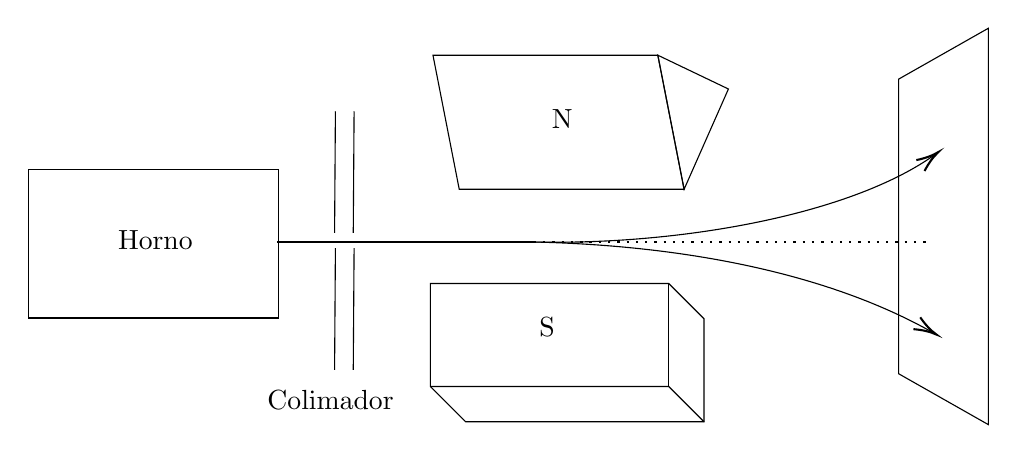
\begin{tikzpicture}[x=0.75pt,y=0.75pt,yscale=-1,xscale=1]
				%uncomment if require: \path (0,480); %set diagram left start at 0, and has height of 480

				%Shape: Cube [id:dp859809843103517] 
				\draw   (233.74,245.6) -- (250.74,262.6) -- (365.6,262.6) -- (365.6,213) -- (348.6,196) -- (233.74,196) -- cycle ; \draw   (365.6,262.6) -- (348.6,245.6) -- (233.74,245.6) ; \draw   (348.6,245.6) -- (348.6,196) ;
				%Shape: Parallelogram [id:dp7759043369492696] 
				\draw   (247.66,150.6) -- (355.99,150.6) -- (343.34,86) -- (235,86) -- cycle ;
				%Shape: Triangle [id:dp6291130251650078] 
				\draw   (355.99,150.6) -- (377.35,102.28) -- (343.34,86) -- cycle ;
				%Shape: Rectangle [id:dp2470860068573859] 
				\draw   (40,141) -- (160.6,141) -- (160.6,212.6) -- (40,212.6) -- cycle ;
				%Straight Lines [id:da5421959652511514] 
				\draw    (188,179) -- (187.6,237.6) ;
				%Straight Lines [id:da5060158615618738] 
				\draw    (197,179) -- (196.6,237.6) ;
				%Straight Lines [id:da4941378235730567] 
				\draw    (188,113) -- (187.6,171.6) ;
				%Straight Lines [id:da2726979507325893] 
				\draw    (197,113) -- (196.6,171.6) ;
				%Straight Lines [id:da27650082873798887] 
				\draw    (160,176) -- (283.6,176) ;
				%Curve Lines [id:da24152820000763586] 
				\draw    (283.6,176) .. controls (353.89,177.58) and (436.92,162.9) .. (477.39,133.5) ;
				\draw [shift={(478.6,132.6)}, rotate = 143.13] [color={rgb, 255:red, 0; green, 0; blue, 0 }  ][line width=0.75]    (10.93,-3.29) .. controls (6.95,-1.4) and (3.31,-0.3) .. (0,0) .. controls (3.31,0.3) and (6.95,1.4) .. (10.93,3.29)   ;
				%Curve Lines [id:da8965916620727498] 
				\draw    (283.6,176) .. controls (353.89,177.58) and (424.18,190.34) .. (476.03,219.71) ;
				\draw [shift={(477.6,220.6)}, rotate = 209.98] [color={rgb, 255:red, 0; green, 0; blue, 0 }  ][line width=0.75]    (10.93,-3.29) .. controls (6.95,-1.4) and (3.31,-0.3) .. (0,0) .. controls (3.31,0.3) and (6.95,1.4) .. (10.93,3.29)   ;
				%Shape: Trapezoid [id:dp5487156542857342] 
				\draw   (502.6,263.99) -- (459.35,239.46) -- (459.35,97.53) -- (502.6,73) -- cycle ;
				%Straight Lines [id:da6387439215210671] 
				\draw  [dash pattern={on 0.84pt off 2.51pt}]  (283.6,176) -- (473.6,176) ;


				% Text Node
				\draw (82,169) node [anchor=north west][inner sep=0.75pt]   [align=left] {Horno};
				% Text Node
				\draw (291,111) node [anchor=north west][inner sep=0.75pt]   [align=left] {N};
				% Text Node
				\draw (285,211) node [anchor=north west][inner sep=0.75pt]   [align=left] {S};

				% Text Node
				\draw (154,246) node [anchor=north west][inner sep=0.75pt]   [align=left] {Colimador};

			\end{tikzpicture}
		}
		\caption{Experimento de Stern-Gerlach}
		\label{fig:stern-gerlach}
	\end{figure}

\end{frame}

\begin{frame}[c]
	\frametitle{Kets y Bras}
	Teoría de kets y bras
\end{frame}

\begin{frame}[c]
	\frametitle{Operadores}
	text
\end{frame}

\begin{frame}[c]
	\frametitle{Principio de incertidumbre}
	text
\end{frame}

\begin{frame}[c]
	\frametitle{Cambio de base}
	text
\end{frame}

\begin{frame}[c]
	\frametitle{Matriz de densidad}
	text
\end{frame}

\begin{frame}[c]
	\frametitle{Ecuación de Schödinger}
	text
\end{frame}

\begin{frame}[c]
	\frametitle{Evolución temporal}
	text
\end{frame}

\begin{frame}[c]
	\frametitle{Imagenes de la MC}
	text
\end{frame}

\begin{frame}[c]
	\frametitle{Oscilador armónico cuántico (OAC)}
	text
\end{frame}

\begin{frame}[c]
	\frametitle{Operadores escalera}
	text
\end{frame}

\begin{frame}[c]
	\frametitle{Estados número del OAC}
	text
\end{frame}

\begin{frame}[c]
	\frametitle{Operadores cuadratura}
	text
\end{frame}

\begin{frame}[c]
	\frametitle{Óptica cuántica}
	text
\end{frame}

\section{Cuantización campo EM}

\begin{frame}[c]
	\frametitle{Ecuaciones de Maxwell}
	text
\end{frame}

\begin{frame}[c]
	\frametitle{Ecuación de onda}
	text
\end{frame}

\begin{frame}[c]
	\frametitle{Solución a la ecuación de onda}
	Repasar teoría de EDP's, EDO's, solución particular y homogénea
\end{frame}

\begin{frame}[c]
	\frametitle{Condiciones de la función de onda}
	text
\end{frame}

\begin{frame}[c]
	\frametitle{Condiciones de la función de onda}
	text
\end{frame}

\begin{frame}[c]
	\frametitle{Soluciones a los campos}
	text
\end{frame}

\begin{frame}[c]
	\frametitle{Energía electromagnética}
	text
\end{frame}

\begin{frame}[c]
	\frametitle{Cuantización del campo}
	text
\end{frame}

\section{Compresión y desplazamiento}

\begin{frame}[c]
	\frametitle{Propiedades de los estados número}
	text
\end{frame}

\begin{frame}[c]
	\frametitle{Fasores}
	text
\end{frame}

\begin{frame}[c]
	\frametitle{Estados coherentes}
	text
\end{frame}

\begin{frame}[c]
	\frametitle{Propiedades de los estados coherentes}
	text
\end{frame}

\begin{frame}[c]
	\frametitle{Simetrías y grupos}
	text
\end{frame}

\begin{frame}[c]
	\frametitle{Grupos de Lie}
	text
\end{frame}

\begin{frame}[c]
	\frametitle{Álgebra de Lie}
	text
\end{frame}

\begin{frame}[c]
	\frametitle{Operador desplazamiento}
	text
\end{frame}

\begin{frame}[c]
	\frametitle{Propiedades del operador desplazamiento}
	text
\end{frame}

\begin{frame}[c]
	\frametitle{Operador compresión}
	text
\end{frame}

\begin{frame}[c]
	\frametitle{Estado comprimido ideal}
	text
\end{frame}

\section{Función de Wigner}

\begin{frame}[c]
	\frametitle{Teoría de función de Wigner}
	text
\end{frame}

\begin{frame}[c]
	\frametitle{Función de Wigner para estados coherentes}
	text
\end{frame}

\section{Amplificador paramétrico}

\begin{frame}[c]
	\frametitle{Óptica no lineal}
	text
\end{frame}

\begin{frame}[c]
	\frametitle{Parametric down conversion}
	text
\end{frame}

\begin{frame}[c]
	\frametitle{Amplificador paramétrico}
	text
\end{frame}

\begin{frame}[c]
	\frametitle{Diagonalización del AP}
	text
\end{frame}

\begin{frame}[c]
	\frametitle{Estado inicial}
	text
\end{frame}

\begin{frame}[c]
	\frametitle{Función de Wigner del campo}
	text
\end{frame}

\begin{frame}[c]
	\frametitle{Expresión paramétrica de la función de Wigner}
	text
\end{frame}

\begin{frame}[c]
	\frametitle{Resultados}
	text
\end{frame}

\begin{frame}[c]
	\frametitle{Conclusiones}
	text
\end{frame}

\begin{frame}[c]
	\centering ¡Gracias por su atención!
\end{frame}

\end{document}






